%!TEX root = ../dokumentation.tex

% Kapitel über Sender-Schaltung, Signalerzeugung
% Idee, Umsetzung etc


\chapter{Sender} %TODO Sender Einleitung
Der Ultraschallsender wird durch ein $40 kHz$-Signal angeregt und erzeugt einen Schallkegel mit etwa $80^\circ$ Abstrahlwinkel. Der Schallpegel sollte dabei möglichst hoch sein, um die erfolgreiche Signalauswertung des reflektierten Signals auch über weite Distanzen und geringen Reflexionsfaktoren zu ermöglichen. Es wird empfohlen, den Sender mit einem Rechtecksignal anzusteuern. Durch sein sehr schmales Spektrum/Frequenz (FIXME) schwingt er dennoch sinusförmig ohne Oberwellen zu erzeugen und nimmt dabei am meisten Energie auf. (FIXME bei gleichbleibender Amplitude im vgl zu anderen Signalen/Sinus). Weiter mit Kapazität des Senders


\section{Signalerzeugung}
Das Rechtecksignal wird von dem Mikrocontroller erzeugt. Er besitzt einen Hardwarezähler, der mit einem Ausgangspin verbunden werden kann. Damit lässt sich ein präzises Signal erzeugen, ohne die Rechenleistung des Controllers einzuschränken.\\
Der Sender hat eine maximale Spitze-Spitze-Spannung von $U_{SS} = 20V$, das ausgegebene Signal des Mikrocontrollers wechselt jedoch nur zwischen $0V$ und $5V$. Die Sendeleistung wäre zu schwach, außerdem sollte der Ausgang des Mikrocontrollers nicht direkt belastet werden, da er nur sehr begrenzt Strom liefern kann. Aus diesen Gründen wurden mehrere Sendeverstärker entwickelt und untersucht, ob sie geeignet sind.



\section{Erste Schaltung: Verstärkung mit Operationsverstärker}
\subsection{Idee} % FIXME Differenzverstärker
Mithilfe eines Operationsverstärkers lassen sich einfach Spannungen verstärken. Mit der Komparatorschaltung kann das $0/5V$-Signal auf $-10/+10V$ umgesetzt werden. Gewählt wurde der Operationsverstärker \textit{LM258}, da seine Spannungsversorgung sehr hoch gewählt werden kann und er eine Bandweite von $1.1MHz$ hat, was für diese Zwecke ausreichen sollte.
\begin{figure}[H]
\centering
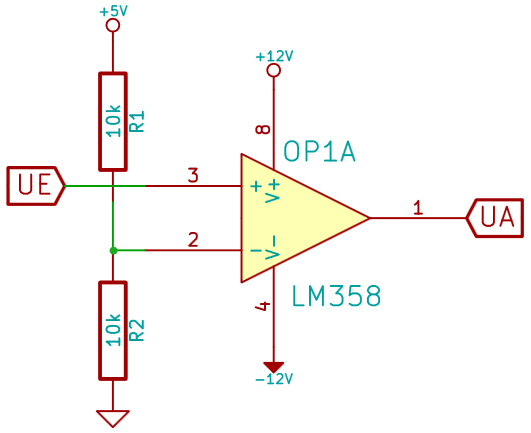
\includegraphics[scale=0.5]{images/komparatorschaltung.jpg}
\caption{Einfache Komparatorschaltung zum Umsetzen der Spannungen} \label{img:I1} %TODO: LM258/358
\end{figure}

\subsection{Problematik}
Bereits bei der Planung der Schaltung wurde befürchtet, dass der maximale Strom des Operationsverstärkers für ein scharfes Signal sehr knapp dimensioniert ist ($I_{Source}=30mA; I_{Sink}=40mA$). Nimmt man an, der Operationsverstärker besitzt einen Ausgangswiderstand von $0 \Omega$ und die Ladespannung beträgt $20V$, ist die Zeit zum vollständigen Laden des Senders:
\begin{equation}
t=\frac{Q}{I}=\frac{C*U}{I}=\frac{2.55nF*20V}{30mA}=1.7\mu s
\end{equation}
Im Vergleich zur Pulsdauer von $12.5\mu s$ ist dieser Wert in Ordnung. Allerdings besitzt nur ein idealer Operationsverstärker einen $0\Omega$-Ausgangswiderstand und der Sender ist auch kein idealer Kondensator. Deshalb wurde erwartet, dass die Flanken etwas abgeflacht werden.\\
Tatsächlich wurde jedoch ein viel wichtigerer Wert im Datenblatt übersehen. Die \textit{Slew Rate} gibt an, wie schnell sich die Spannung des OPs ändern kann. Beim \textit{LM258} beträgt sie $0.6V/\mu s$. Das Ausgangssignal entsprach aus diesem Grund einem Dreiecksignal und schwankte nur um wenige Volt.
% Bild von Simulation
\begin{figure}[H] %TODO: Kontrast von Bild erhöhen
\centering
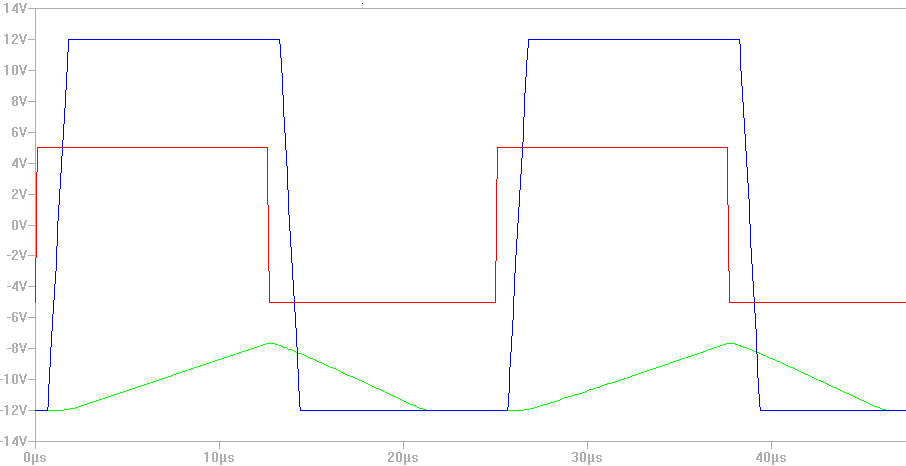
\includegraphics[scale=0.6]{images/signalverlauf_opamps.png}
\caption{Simulierter Signalverlauf von zwei Operationsverstärkern. Rot: Ansteuersignal. Grün: Slew-Rate $0.6V/\mu s$. Blau: Slew-Rate $20V/\mu s$.} \label{img:I2}
\end{figure}

\subsection{Fazit}
Die Spannungsverstärkung mit dem Operationsverstärker \textit{LM258} hat sich als nicht praktikabel herausgestellt, da er zu langsam reagiert. Für diese Zwecke können jedoch spezielle \textit{Komparatoren} verwendet werden, die sich wie Operationsverstärker verhalten, nur viel schneller und ungenauer sind. Die Genauigkeit spielt beim Umschalten keine Rolle.\\
Nach dieser Feststellung wurden Schaltungen mit Transistoren untersucht, da sie höhere Leistungen und schnellere Reaktionszeiten zulassen. Die Lösung mit Komparator wurde für den Fall, dass die weiteren Schaltungen keine befriedigende Ergebnisse liefern, für später aufgehoben.


\section{Zweite Schaltung: Verstärkung mit Transistor}



\section{Dritte Schaltung: Gegentaktausgangsstufe, Push/Pull}




